%Flo
\section{Recovery Concepts}

\subsection{Recovery Outline and Categorization of Recovery Algorithms}

Recovery from transaction failures means that the DB is restored to the most recent consistent state before the time of failure. To do this, the changes made by DB operations are kept in the \textbf{system log}. If there is extensive damage to a wide portion of the DB due to catastrophic failure, e.g. disk crash, the recovery method restores a past copy of the DB. Otherwise, the recovery strategy is to identify any changes that may cause inconsistency in the DB. \\

We distinguish between two main policies for recovery from non-catastrophic failures~:
\begin{itemize}
    \item \textbf{Deferred update} techniques update the DB only \textit{after} a transaction commits. These are discussed in section~\ref{chap22-deferred}.
    \item \textbf{Immediate update} techniques. The DB may be updated \textit{before} the transaction reaches its commit point. These are discussed in section~\ref{chap22-immediate}
\end{itemize}

Both techniques may involve UNDO and REDO operations. These apply to DB operations. They are \textbf{idempotent}, i.e. executing a specific operation multiple times is equivalent to executing it just once.

\subsection{Caching of Disk Blocks}
The \textbf{DBMS cache} is a collection of in-memory buffers. As the page tables in the operating system, there is a \textbf{directory} for the cache  to keep track of which items are in the buffers. Associated with each buffer is a \textbf{dirty bit}. As in the operating system it is used to denote a buffer that has been modified since its content has been brought from disk. Another bit is needed~: the \textbf{pin-unpin} bit. A page in the cache is \textbf{pinned} if it cannot be written back to disk as yet. It used by the recovery protocol to restrict certain buffer pages. \\

Two main strategies can be employed when flushing a modified buffer back to disk.

\begin{itemize}
    \item \textbf{In-place updating} writes the buffer to the \textit{same} original disk location, thus overwriting the old value.
    \item \textbf{Shadowing} writes the buffer at a \textit{different} disk location, thus multiple versions of the data item are kept on disk.
\end{itemize}

The old value of the data item before updating is called the \textbf{before image} (\textbf{BFIM}) and the new value after updating is called the \textbf{after image} (\textbf{AFIM}).


\subsection{Write-Ahead Logging, Steal/No-Steal, and Force/No-Force}
In an in-place updating scheme, the BFIM of the data item is recorded in the appropriate log entry and that log entry is flushed to disk before the BFIM is overwritten with the AFIM on disk. This process is called \textbf{write-ahead logging} and is necessary so we can UNDO the operation if needed. \\

\begin{samepage}
There are two types of log entry~:

\begin{itemize}
    \item \textbf{REDO-type log entry} includes the \textit{new} value AFIM of the item.
    \item \textbf{UNDO-type log entry} includes the \textit{old} value BFIM of the item.
\end{itemize}
\end{samepage}

If a cache buffer page updated by a transaction $T$ \textit{cannot} be written to disk before $T$ commits, the recovery method is called a \textbf{no-steal approach}. The pin-unpin bit is pinned. If the recovery protocol allows writing an updated buffer \textit{before} $T$ commits, it is called \textbf{steal}. Note that the \textit{no-steal} rule means that UNDO will never be needed during recovery. \\

If all pages updated by $T$ are immediately written to disk \textit{before} $T$ commits, the recovery protocol is called a \textbf{force approach}. Otherwise it is called \textbf{no-force}. Note that the \textit{force} rule means that REDO will never be needed during recovery. \\

\begin{samepage}
The \textbf{write-ahead logging} (\textbf{WAL}) protocol is used to permit recovery when in-place updating is used. It works as follows~:

\begin{itemize}
    \item[1.] The BFIM of an item $X$ cannot be overwritten by its $AFIM$ on disk until all UNDO-type log entries have been force-written to disk.
    \item[2.] The transaction $T$ cannot commit until all the REDO-type and UNDO-type log entries for $T$ have been force-written to disk.
\end{itemize}
\end{samepage}

\subsection{Checkpoints in the System Log and Fuzzy Checkpointing}
A \textbf{checkpoint} is a type of entry in the log, it is of the form \texttt{[checkpoint, \textit{list of active transactions}}. Taking a checkpoint consists of the following actions~:

\begin{itemize}
    \item[1.] Suspend execution of transactions.
    \item[2.] Force-write all main memory buffers that have been modified to disk.
    \item[3.] Write a [\texttt{checkpoint}] record to the log, and force-write the log to disk.
    \item[4.] Resume executing transactions.
\end{itemize}

To reduce the time during which transactions are suspended, the system can use \textbf{fuzzy checkpointing}. It consists of writing a \texttt{[begin\_checkpoint]} record at the beginning of step 2 and a \texttt{[end\_checkpoint]} record at the end of step 2. As soon as the first record is written, all transactions can be resumed.

\subsection{Transaction Rollback and Cascading Rollback}

If a transaction $T$ fails after updating the DB but before it commits, it may be necessary to \textbf{roll back} $T$. If $T$ is rolled back, any transaction $S$ that has read the value of some data item $X$ written by $T$ must also be rolled back. Similarly, once $S$ is rolled back, any transaction $R$ that has read the value of some data item $Y$ written by $S$ must also be rolled back, and so on. This phenomenon is called \textbf{cascading rollback}. However, almost all recovery mechanisms are designed so that cascading rollback is \textit{never required}. 


\section{NO-UNDO/REDO Recovery Based on Deferred Update}
\label{chap22-deferred}
A typical deferred update protocol can be stated as follows~:

\begin{itemize}
    \item[1.] A transaction $T$ cannot change the DB on disk until it reaches its commit point. Hence, all buffers that have been changed by $T$ must be pinned until $T$ commits. This is a \textit{no-steal} policy.
    \item[2.] A transaction $T$ does not reach its commit point until all its REDO-type log entries are recorded in the log \textit{and} the log buffer is force-written to disk. This is the WAL protocol.
\end{itemize}

So no UNDO is necessary since the DB is never updated on disk until after a transaction commits. A possible recovery algorithm using deferred update in a multiuser environment is the following~: \\

Use two lists of transactions~: the committed transactions $T$ since the \textit{last checkpoint} and the active transactions $T'$. REDO all the WRITE operations of the committed transactions from the log, \textit{in the order in which they were written into the log}. The transactions that are active and did not commit are effectively canceled and must be resubmitted. \\

\label{chap22-redo-proc}
\textbf{Procedure REDO (WRITE\_OP}~: Redoing a \texttt{write\_item} operation consists of examining its log entry [\texttt{write\_item},$T$,$X$,\texttt{new\_value}] and setting $X=\texttt{new\_value}$ in the DB. \\

Note that this protocol is more efficient if we start from the end of the log and redo only the \textit{last update} of each item $X$.

The advantage of this method is that transaction operations never need to be undone. Indeed, $T$ does not record any changes on disk until after it reaches its commit point and so $T$ is never rolled back. Also, $T$ will never read the value of an item that is written by an uncommitted transaction $T'$ so no cascading rollback will occur. \\

The drawback of this approach is that many cache buffers will be pinned and so cannot be replaced before the commit points of the transactions.



\section{Recovery Techniques Based on Immediate Update}
\label{chap22-immediate}
We can distinguish two main categories of immediate update algorithms. \\

\begin{itemize}
    \item[1.] All updates by a transaction $T$ are recorded on disk \textit{before} $T$ commits, so REDO is never needed. Hence this method uses the \textbf{steal/force} strategy.
    \item[2.] If $T$ is allowed to commit before all its changes are written to the DB, we have the general case, known as UNDO/REDO recovery algorithm. In this case, the \textbf{steal/no-force} strategy is applied. This is the most complex technique but also the most commonly used in practice.
\end{itemize}

The recovery procedure using immediate updates for a multiuser environment is presented below. However, we discuss in section~\ref{chap22-aries} a more practical approach known as ARIES.

\begin{itemize}
    \item[1.] Use two list of transactions~: the committed ones since the last \textit{checkpoint} and the active ones.
    \item[2.] Undo all the \texttt{write\_item} of the active transactions, using the UNDO procedure (showed below). They are undone in the reverse of the order in which they were written into the log.
    \item[3.] Redo all the \texttt{write\_item} of the committed transactions, using the REDO procedure (section~\ref{chap22-redo-proc}) in the order in which they were written into the log. 
\end{itemize}

\textbf{Procedure UNDO (WRITE\_OP)} consists of examining its log entry [\texttt{write\_item}, $T$, $X$, \texttt{old\_value}, \texttt{new\_value}] and setting $X=\texttt{old\_value}$.

Note that step 3, as presented for the NO-UNDO/REDO procedure is more efficiently done if we start from the end of the log and redo only the \textit{last update} of each item $X$.



\section{Shadow Paging}
In shadow paging, when a transaction $T$ begins, its \textbf{directory}, i.e. its $n$ cache entries that points to the most recent DB pages on disk, is copied into a \textbf{shadow directory}. During $T$ execution, the shadow directory is never modified. When a \texttt{write\_item} is performed, a new copy of the modified DB page is created~: the old page is not overwritten. Figure~\ref{fig:chap22-shadow} shows a situation during $T$ execution where pages 2 and 5 have been updated. \\

\begin{figure}[h!]
    \centering
    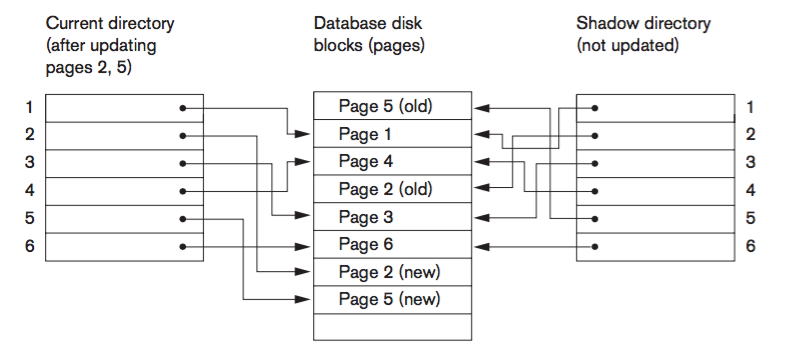
\includegraphics[scale=0.5]{chap22-shadow.png}
    \caption{An example of shadow paging}
    \label{fig:chap22-shadow}
\end{figure}

To recover from a failure during $T$ execution, we free the modified DB pages and discard the current directory. We then reinstate the shadow directory. To commit $T$, we discard the shadow directory. This is a NO-UNDO/NO-REDO technique for recovery. \\



\section{The ARIES Recovery Algorithm}
\label{chap22-aries}
ARIES is a specific scheme used in many of IBM’s relational database products. ARIES uses a steal/no-force approach for writing, and it is based on 3 concepts: \textbf{WAL, repeating history during redo, and logging changes during undo}.\\
\textbf{Repeating history}, means that ARIES will retrace all actions of the database system prior to the crash to reconstruct the database state when the crash occurred. Uncommitted transactions at the time of the crash are undone. \textbf{Logging during undo}, will prevent ARIES from repeating the completed undo operations if a failure occurs during recovery, which causes a restart of the recovery process.\\

The ARIES recovery procedure consists of three main steps: analysis (identity the dirty pages and set of transactions active at the time of the crash), REDO (not only applied to committed transaction: REDO all the logs from a start point to the end), and UNDO (operations of active transactions at the time of the crash are undone).\\

Every log record has an associated log sequence number (LSN) that is increasing and indicates the address of the log record on disk. A log record is written for any of the following actions: updating a page (write), committing a transaction (commit), aborting a transaction (abort), undoing an update (undo) (to avoid the undo to be repeated), and ending a transaction (end).\\

In addition to the log, two tables are needed for efficient recovery: the \textbf{Transaction Table} and the \textbf{Dirty Page Table}, both completed by the analysis phase. The REDO phase starts from the smallest LSN in the Dirty Page Table and proceeds up to the end of the log file. The Transaction Table contains the active transactions. The UNDO phase starts at the log entry from the latest active transaction and proceeds backwards in the log.\\

ARIES uses fuzzy checkpointing.

\section{Recovery in Multidatabase Systems}
A multidatabase transaction, may access to multiple databases. Each DBMS involved in the multidatabase transaction has its own recovery technique and transaction manager. To maintain the atomicity of a multidatabase transaction, it is necessary to have a two-level recovery mechanism: a global recovery manager and the local recovery managers. The global recovery manager usually follows the two-phase commit protocol:
\begin{itemize}
    \item \textbf{Phase 1.} Every local manager sends a message when it has finished the transaction and waits for the response of the global manager before committing. The global manager sends the response to all the local managers when they all said that they were ready to commit. Then the local managers reply with "ok" or "not ok" if it committed successfully of not.
    \item \textbf{Phase 2.} If a transaction has failed, then the global manager sends a message to rollback to all the local managers.
\end{itemize}
So all local databases commit the effect of the transaction or none of them do.

\section{Database Backup and Recovery from Catastrophic Failures}
The recovery techniques we have discussed use the entries in the system log or the shadow directory (both stored on disk) to recover from failure by bringing the database back to a consistent state. The recovery manager of a DBMS must also be equipped to handle more catastrophic failures such as disk crashes. Make frequent backups ! The system log should be backed up more frequently than the whole database to avoid losing all the effects of transactions that have been executed since the last backup. A new log is started after each database backup.

\section{Summary}
The main goal of recovery is to ensure the atomicity of a transaction. If a transaction fails before completing its execution, the recovery mechanism has to make sure that the transaction has no lasting effects on the database.\\

Deferred update techniques postpone the updating of the database on disk until a transaction reaches its commit point. The transaction force-writes the log to disk before recording the updates in the database. It never requires transaction rollback, and recovery simply consists of redoing the operations of transactions committed after the last checkpoint from the log. This leads to the NO-UNDO/REDO algorithm. In contrast, immediate update techniques, where changes to the database are applied on disk before the transaction commits, leads to the UNDO/REDO algorithm.\\

Shadow paging, classified as NO-UNDO/NO-REDO, does not require a log in single-user systems but still needs the log for multi-users systems.\\

Recovery from catastrophic failures is typically done by backing up the database and the log to tape. The log, which is backed up more frequently, can be used to redo operations starting from the last database backup.